\documentclass[12pt]{article}
\usepackage[margin=0.5in]{geometry}
%\documentclass[11pt,preprint]{aastex}
\usepackage{amsmath,amssymb}
\usepackage{natbib}
\setlength{\bibsep}{4.0pt}
\usepackage{graphicx} 
\usepackage{setspace}
\usepackage{float}
\usepackage{subfig}
\usepackage[usenames]{color}
\definecolor{Red}{rgb}{1.00,0.00,0.00}

\newcommand{\degr}{\ensuremath{^\circ}}

\begin{document}
\textbf{PI:} D. J. Schlegel \textbf{Title:} Mass Mapping Abell 2261 with Kinematic Weak Lensing \textbf{ID:} 2014A\_U051D

\section{Science Justification}


\subsection{Cluster Mass Mapping}

The mass distribution in galaxy clusters is a crucial test of our cosmological paradigm. Total halo masses probe the amplitude of matter fluctuations and growth of structure in the Universe, and the abundance of substructure within halos is sensitive to the history of hierarchical assembly and potentially the interaction cross-section of dark matter \citep[e.g.,][]{Natarajan2002a, Natarajan2002b, Voit2005, Clowe2006}. Gravitational lensing has played an important role in mapping dark matter within halos, primarily by exploiting the distortion of images of background galaxies. On small scales inside lensing clusters, strong distortions produce extended arcs and multiple images enabling the production of detailed mass maps, while on larger scales the distortions are weaker and require averaging the shapes of many background galaxies over a broad area to extract a shear signal.

We propose to map the projected mass distribution in the massive cluster Abell 2261 with a new lensing techinque that uses kinematic measurements of background sources to drastically improve the signal-to-noise (${\rm S/N}$) per galaxy. The typical weak lensing shear signal averaged within the virial radius of a massive cluster ($g_t\sim0.05$) is small compared to the distribution of intrinsic shapes in imaging (which has scatter $\sigma_\gamma\sim0.25$). Kinematic information can be used to infer the intrinsic shape and orientation of the background galaxies, potentially reducing the shape noise per galaxy by a factor of ten. This enables ${\rm S/N}\gtrsim1$ measurements of shear per galaxy. With such precision we will improve the spatial resolution of mass maps and extend the precision of strong lensing out to the weak regime near the virial radius of the cluster.  We plan to create a joint mass reconstruction combining our kinematic lensing measurements with existing shear measurements from Suprime-Cam and HST data to exploit the synergies between the denser sampling of the mass field with traditional weak lensing and the higher individual S/N from the kinematic measurements. We discuss the kinematic technique and its potential for improving both the precision and accuracy of future large-scale lensing experiments in the next section. Additionally, the slit spectra taken at two position angles for hundreds of sources behind A2261 will provide two-dimensional kinematics of emission line disk galaxies, greatly enhancing the sample size at that redshift for studying evolution of galaxy kinematics and the Tully-Fisher relation (TFR).

\subsection{Kinematic Weak Lensing}

The utility of kinematic maps for weak lensing was originally described by \citet{Blain2002} and \citet{Morales2006}, who forecasted constraints from high ${\rm S/N}$, high spatial resolution observations with future radio arrays. The basic idea for the kinematic shear observables is described in Figure~\ref{fig:vmaps}. In an image, an inclined rotating circular disk has elliptical isophotes. When the image of this galaxy is sheared, the isophotes remain elliptical (in the weak shear limit, ($|g_t|\ll1$) with a new axis ratio and position angle. New photometric axes are inferred from this ellipse in the sheared image, and information about the original axes is lost. The case is different however, with kinematic measurements. The unsheared circular disk has kinematic axes that are perpendicular to one another and are aligned with the unsheared photometric axes. This cross shape becomes skewed when the velocity map is sheared; the kinematic axes are no longer perpendicular and they are misaligned with the photometric axes inferred from the sheared isophotal ellipse in the imaging data.

Full two-dimensional kinematic maps are not required for this measurement, and our approach adds to the previous discussion by incorporating information from the TFR, an empirical scaling relation for disk galaxies between their luminosity and circular velocity $v_{\rm circ}$. With slit spectroscopy, the measured amplitude of a rotation curve is related to the true circular velocity by $v_{\rm obs} = v_{\rm circ} \sin i$, where $i$ is the inclination of the disk toward the observer. Thus the offset between $v_{\rm obs}$ and $v_{\rm circ}$ predicted from the TFR gives a kinematic estimate of $\sin i$. A photometric estimate of $\sin i$ can be obtained from the ellipticity of the image. The difference between both estimates of $\sin i$ gives an estimate of the shear.

For ideal circular disks, the shear can be measured to arbitrary precision, limited only by the spatial and spectral resolution of the data. In practice, the precision of the shear measurement is limited by the intrinsic scatter of the TFR, which arises from effects including disk noncircularity, bulges, warps, and winds. After inclination correction, estimates for the intrinsic fractional scatter in $v_{\rm circ}$ at fixed luminosity or stellar mass are typically $0.05-0.06\,{\rm dex}$ both locally and to $z\sim1.3$ \citep{Reyes2011, Miller2011}. For a properly weighted estimator of the galaxy shape based on the TFR offset, this scatter maps to an uncertainty in the intrinsic galaxy ellipticity of only $\sigma_{\epsilon, {\rm TFR}}=0.015$. This should be compared to the intrinsic shape noise for pure disks $\sigma_{\epsilon, {\rm disks}}=0.59$ and for real imaging surveys $\sigma_{\epsilon, {\rm im}}\approx0.4$, and is related to the shear noise through $\sigma_\epsilon / \sigma_\gamma \approx 2(1-\sigma_\epsilon^2)$\citep{Bernstein2002, Hirata2004}. The scatter in kinematic shape estimates is also sensitive to measurement errors in $v_{\rm circ}$, as shown in Figure~\ref{fig:shapeNoise}. In general, rotation curve errors of $<10\,{\rm km/s}$ reduce the disk galaxy shape noise by an order of magnitude compared with imaging alone.

\subsection{A Pilot Study for Future Dark Energy Experiments}

In addition to its uses in mapping individual structures, statistical weak lensing over wide fields is also a major science driver for several ongoing and future cosmology experiments, ranging from the ongoing Dark Energy Survey and Kilo-Degree Survey projects to space missions like Euclid and the Wide-Field Infrared Survey Telescope. The errors in these surveys are likely to be dominated by systematic errors arising from the necessity of using photometric redshifts for the sources and the difficulties in obtaining unbiased shape measurements for galaxies near the detection limit. In addition to its primary science goals described above, this proposal is also a pilot study, informing our understanding of the viability of kinematic weak lensing over wide fields with the next generation of fiber-fed massively multi-object spectrographs. Instruments such as the planned MS-DESI or Subaru Prime Focus spectrographs are expected to achieve target densities similar to those we propose to obtain here, but over thousands of square degrees. If even crudely resolved kinematics can be obtained by these instruments, it may be possible perform wide-field kinematic weak lensing measurements that significantly exceed even future space missions in their weak lensing signal-to-noise, while avoiding the aforementioned sources of systematic bias that remain highly problematic for existing lensing studies.

\subsection{2-d Disk Kinematics at $z\approx0.8$}

This project will substantially increase the sample size of galaxies with measured two-dimensional kinematics at $z=0.6-1.2$. Existing IFU surveys at these redshifts include IMAGES \citep[N=63;][]{Flores2006, Yang2008} and MASSIV \citep[N=84;][]{Contini2012}. There are some discrepancies between the TFR inferred from these IFU data and from DEIMOS slit spectra \citep[e.g. Figure 12 of][]{Kassin2012}. Our data will help resolve whether these offsets are due to differences in sample selection, slit position angle offsets, or unrelaxed kinematics which are easier to identify in two-dimensions. With [OII], H$\beta$, and [OIII] for our primary targets (depending on redshift) and H$\alpha$ for any interlopers from the foreground cluster at $z=0.225$, we can also probe the spatial distribution of line emission, metallicity, and star-formation, allowing a better understanding of feedback, shocks, outflows, and mergers. The multi-wavelength HST imaging available in the inner portion of the field will enable precise bulge-disk decomposition for improved kinematic modeling. Our sample is selected to lie behind a massive cluster making it unique among these data sets for our lensing goals, but is sufficiently distant that the local environment of our targets will be a fair sample for comparison with other field studies.

\newpage

\begin{figure}[H]
\begin{center}
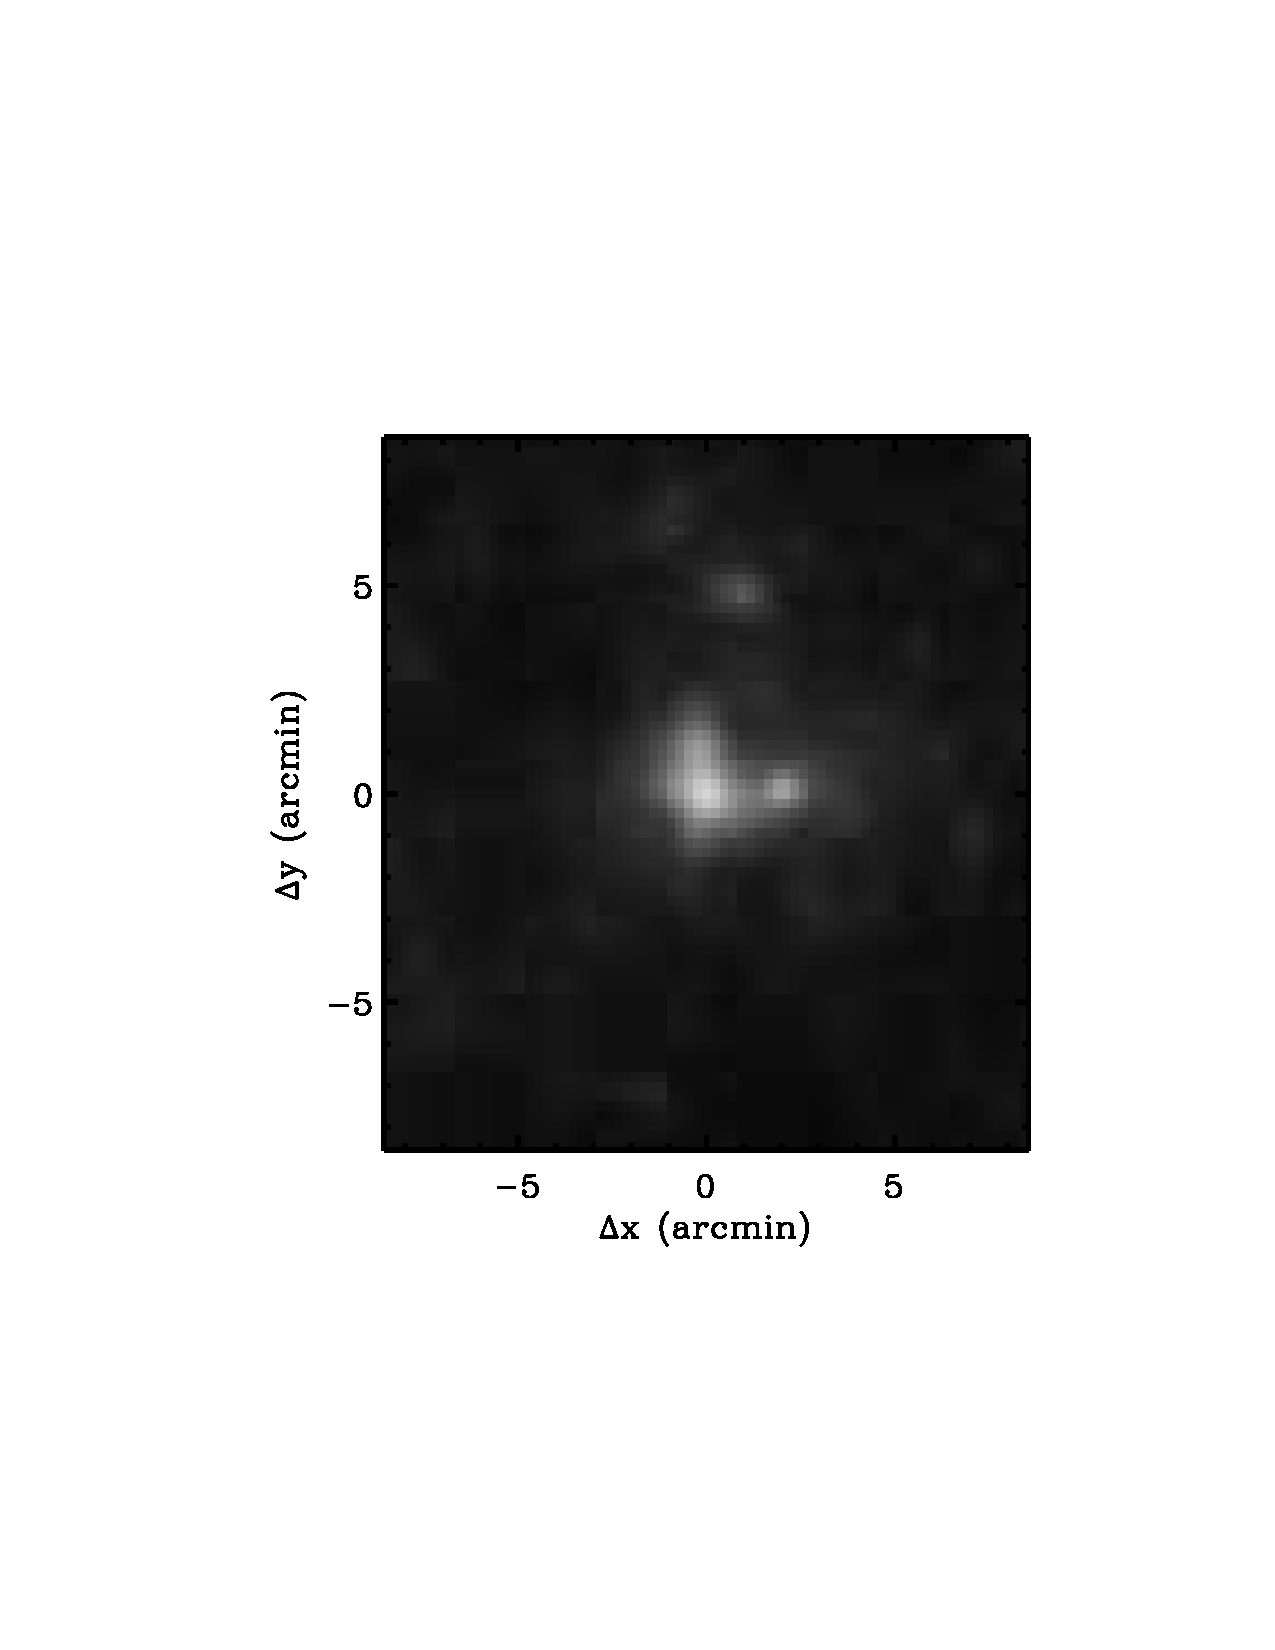
\includegraphics[width=0.3\linewidth,bb= 160 150 500 650,clip]{Plots/shear_map_kappa.pdf}
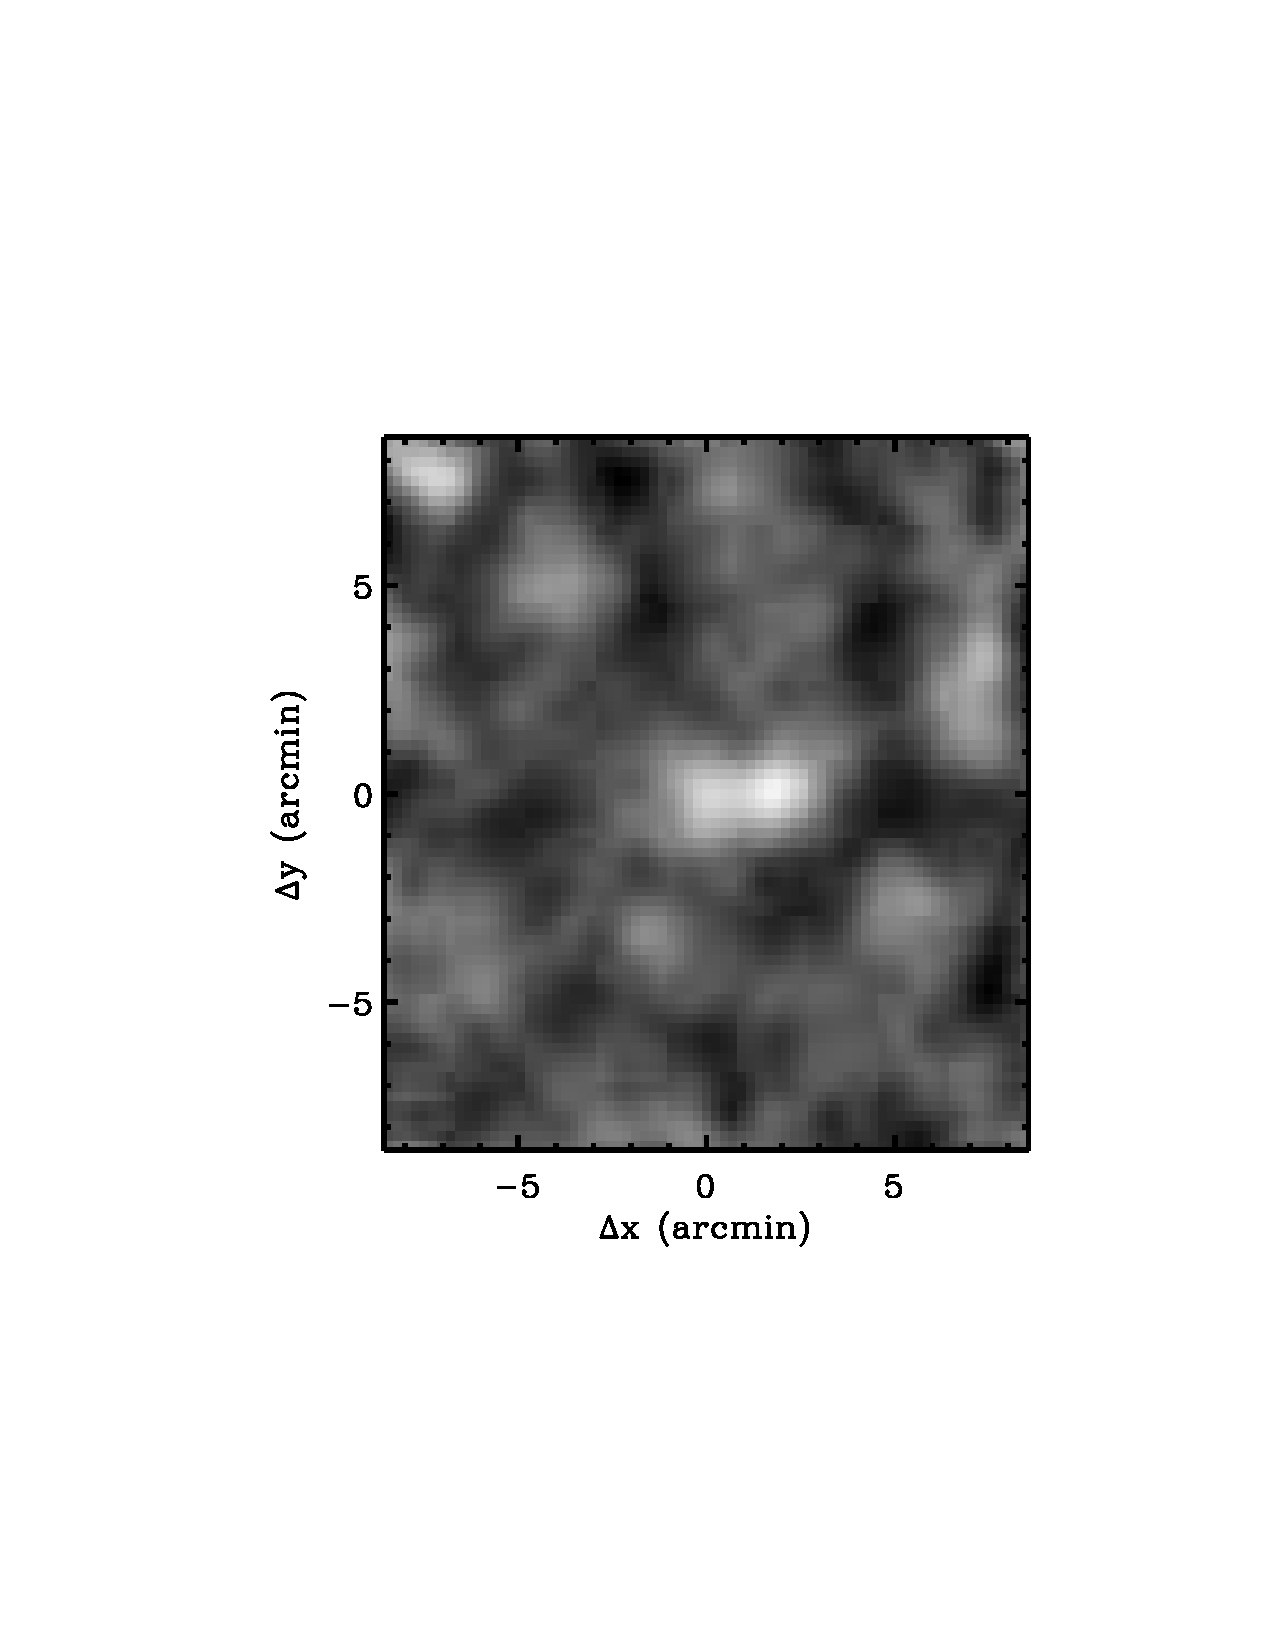
\includegraphics[width=0.3\linewidth,bb= 160 150 500 650,clip]{Plots/shear_map_subaru.pdf}
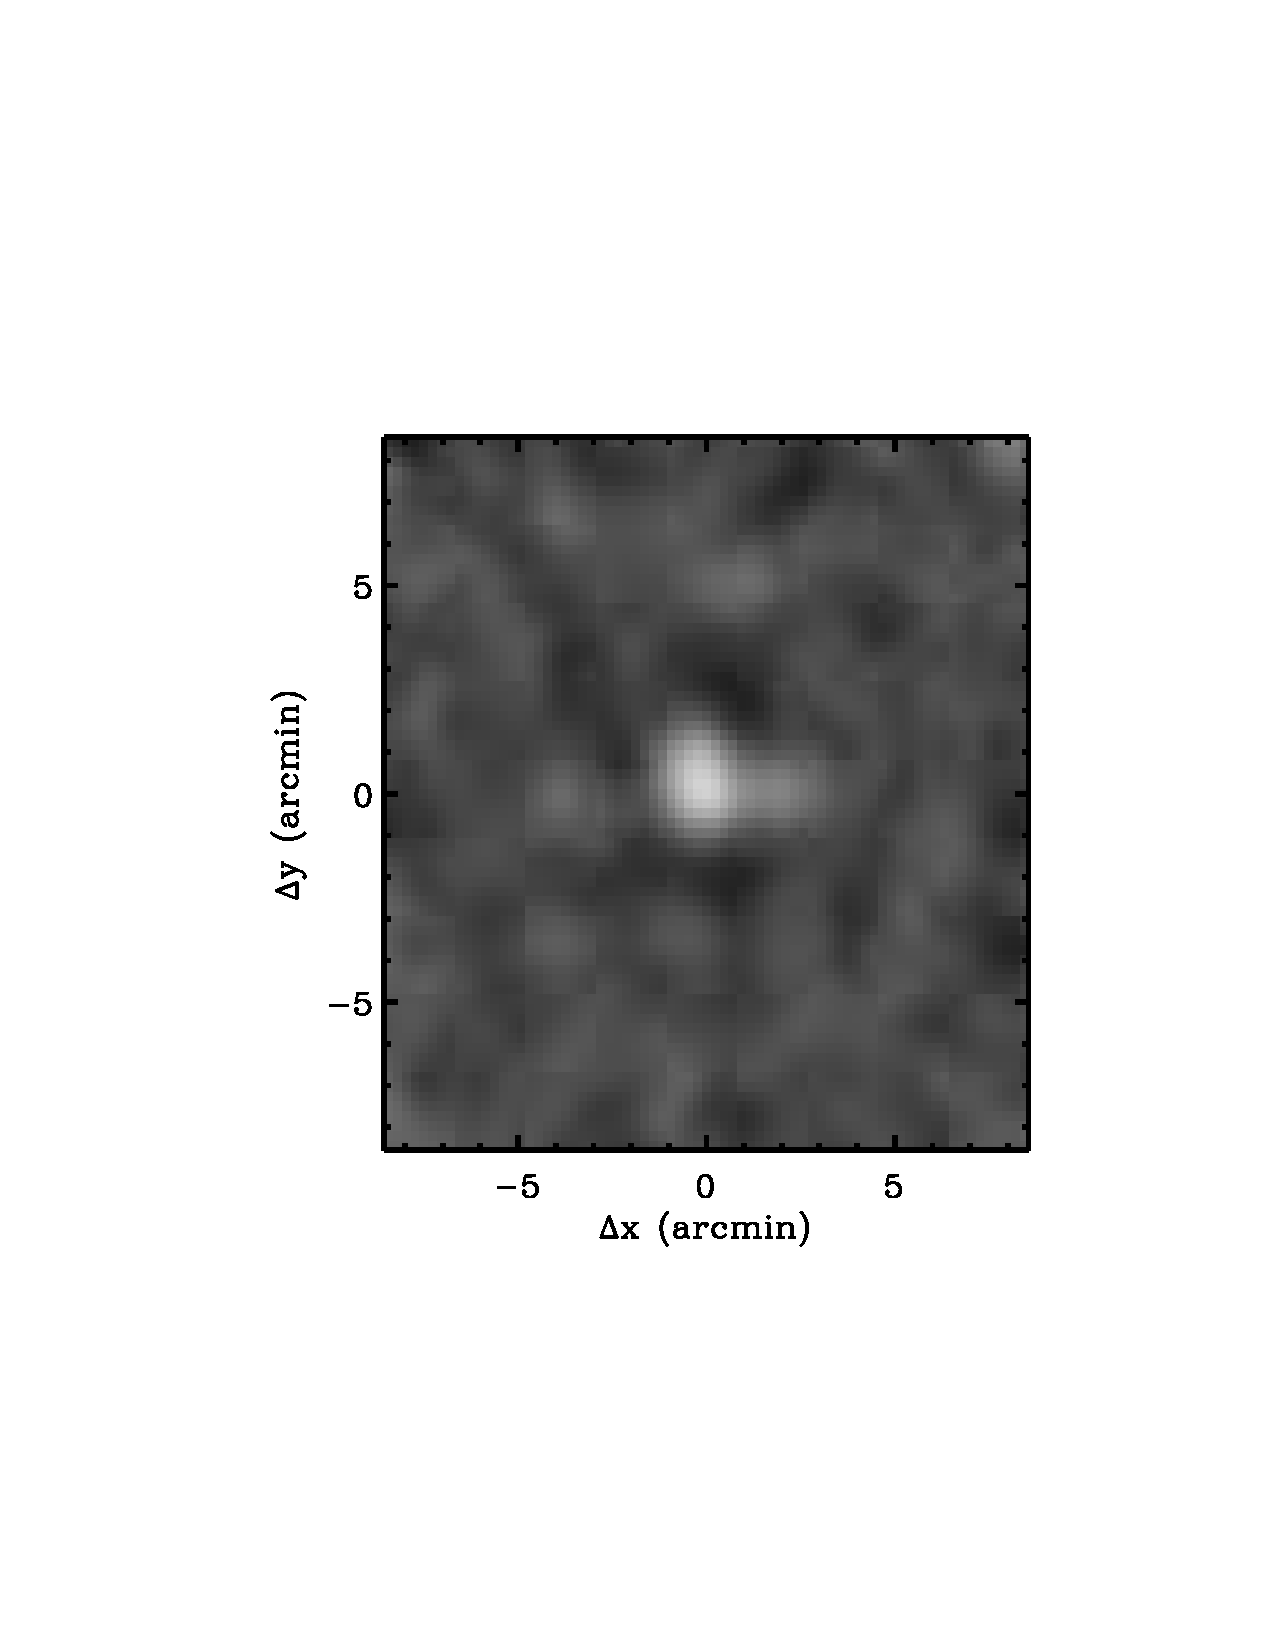
\includegraphics[width=0.3\linewidth,bb= 160 150 500 650,clip]{Plots/shear_map_tf.pdf}
\caption{\footnotesize {\bf Left:} mass map, from \citet{Vale2003} simulations, zoomed in on an extended $~10^{15}M_{\odot}$ cluster. {\bf Center:} Aperture mass map with shape noise properties equivalent to existing Subaru observations of A2261. {\bf Right:} Aperture mass map with shape noise properties equivalent to proposed TFR lensing survey. Aperture scale is tuned for the latter two to optimize signal-to-noise and resolution. Peak observed $\kappa$ values are approximately .07.}
\label{fig:massmaps}
\end{center}
\end{figure}


\begin{figure}[H]
\begin{center}
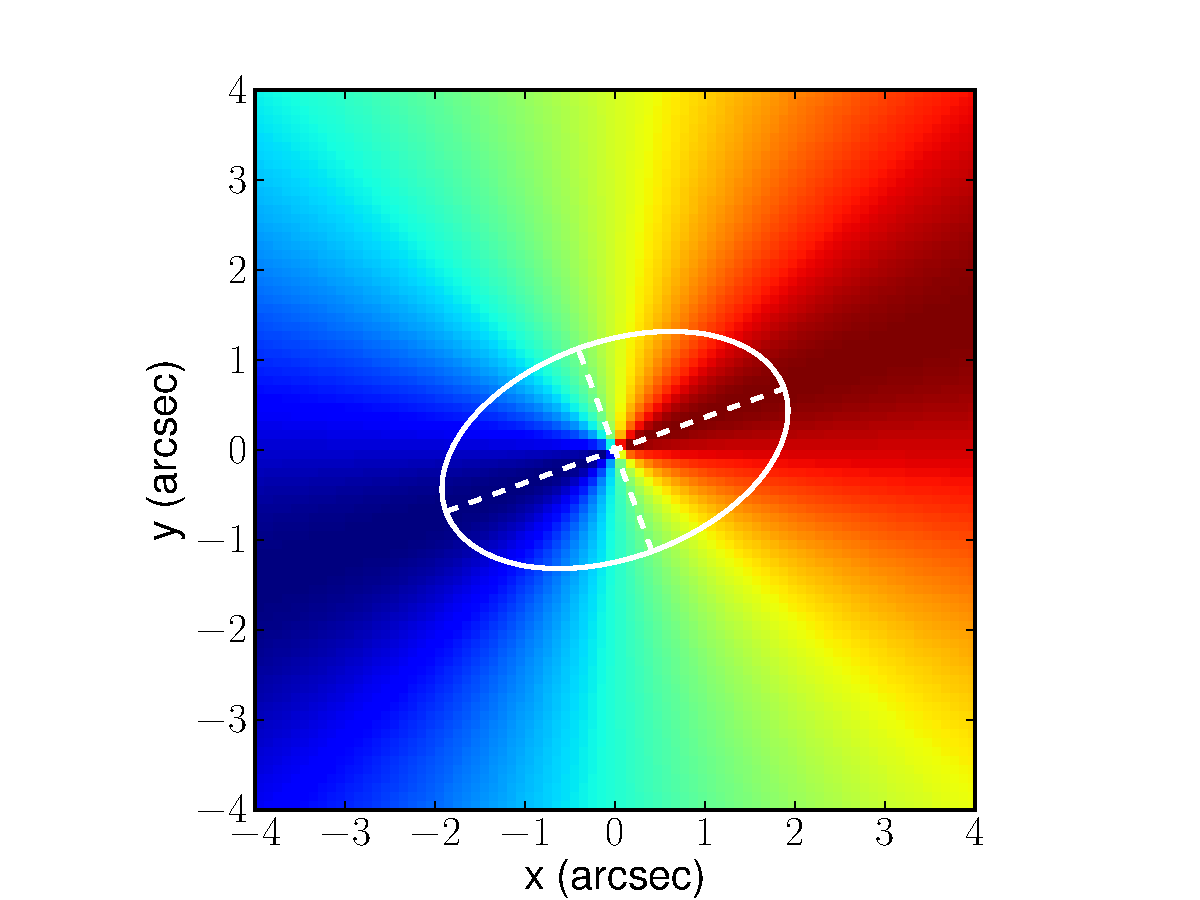
\includegraphics[width=0.49\linewidth]{Plots/fig1a.pdf}
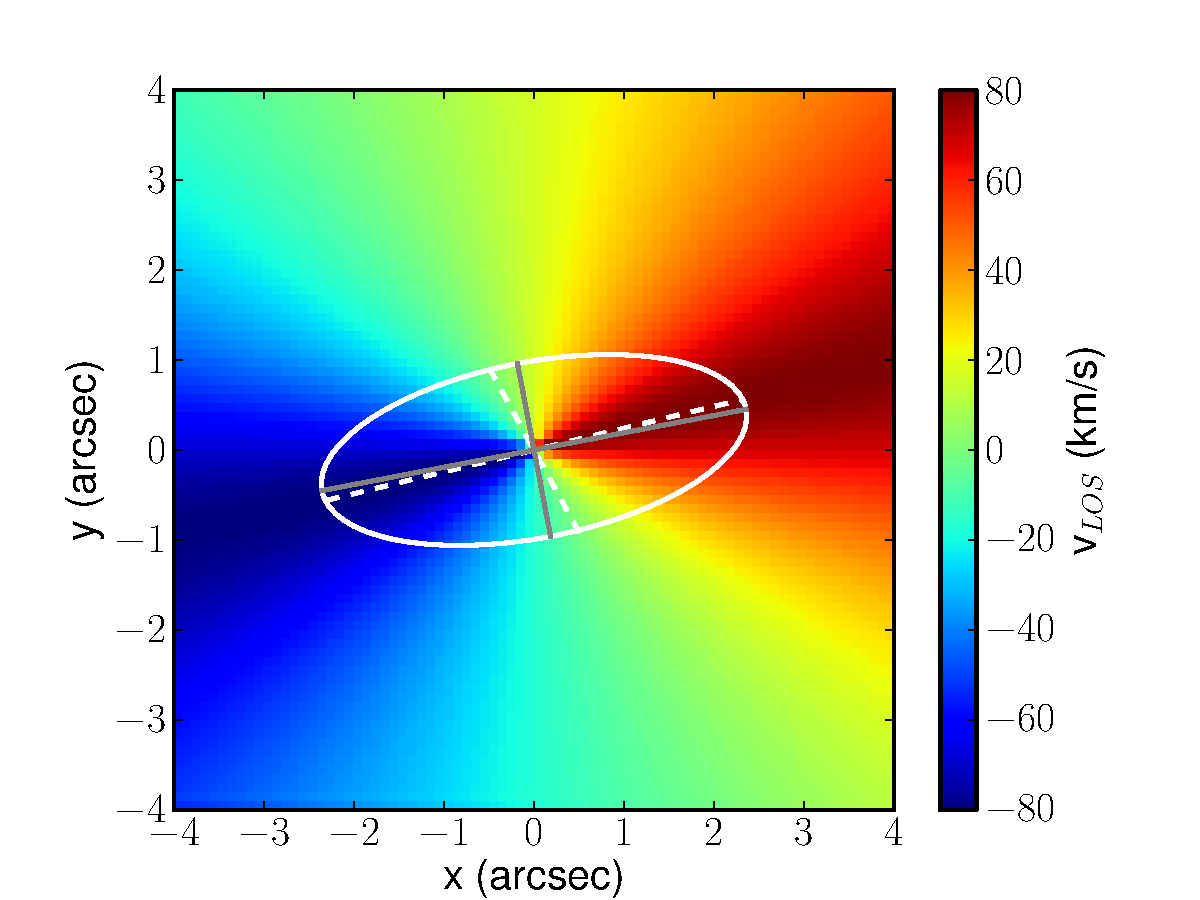
\includegraphics[width=0.49\linewidth]{Plots/fig1b.pdf}
\caption{Effects of shear on kinematic maps of an inclined disk galaxy (Left: unsheared, Right: sheared). Colors show velocity map, and white contours show a single image isophote. A shear applied at $45\degr$ to the disk major axis misaligns the kinematic axes (white dashed lines) and photometric axes (gray solid lines). Effect is illustrated for a shear with amplitude $|\gamma|$=0.1.}
\label{fig:vmaps}
\end{center}
\end{figure}

\begin{figure}[H]
  \parbox{0.45\linewidth}{
    \begin{center}
    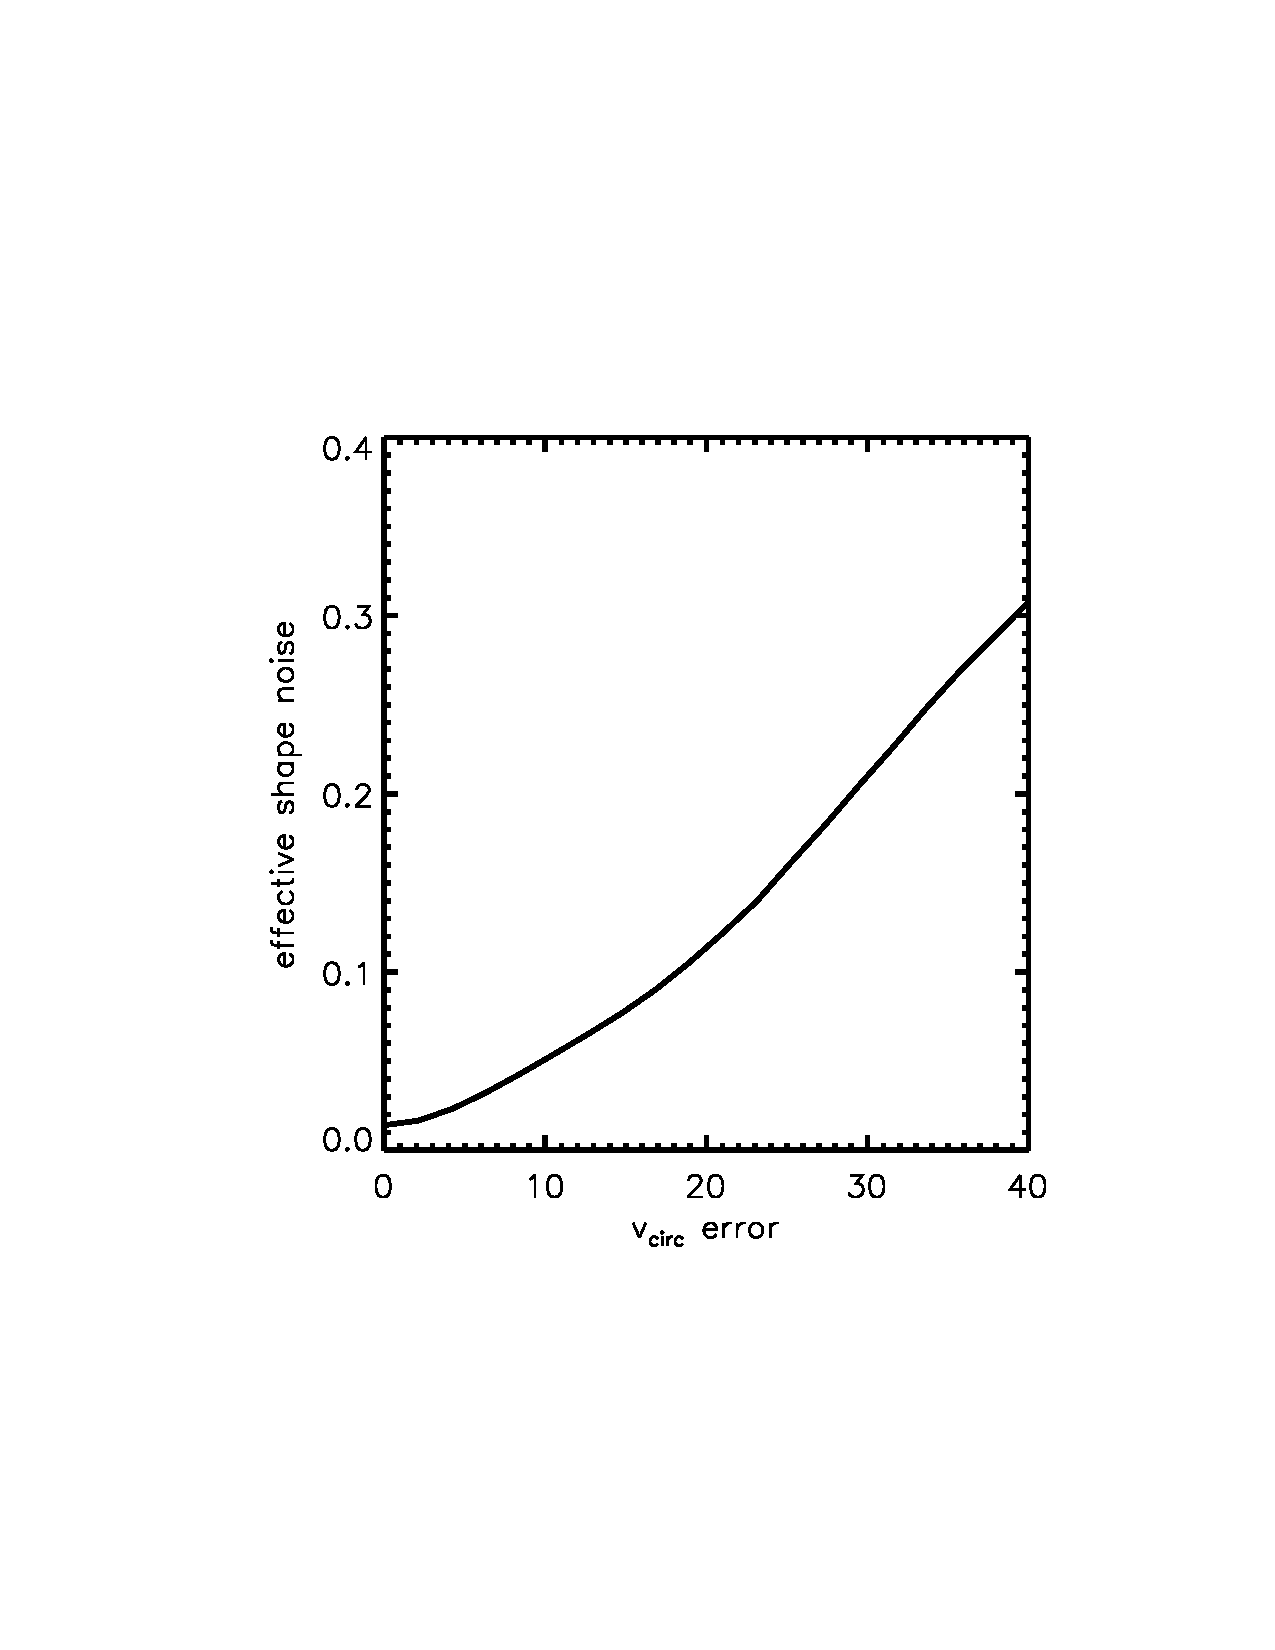
\includegraphics[width=\linewidth, bb= 150 150 590 650,clip]{Plots/vcirc_error.pdf}
    \caption{\footnotesize Effective shape noise $\sigma_{TF}$ as a  function of the
      measurement error on the disk circular velocity.}
    \label{fig:shapeNoise}
    \end{center}
  }
  \qquad
  \begin{minipage}{0.45\linewidth}
    \begin{center}
    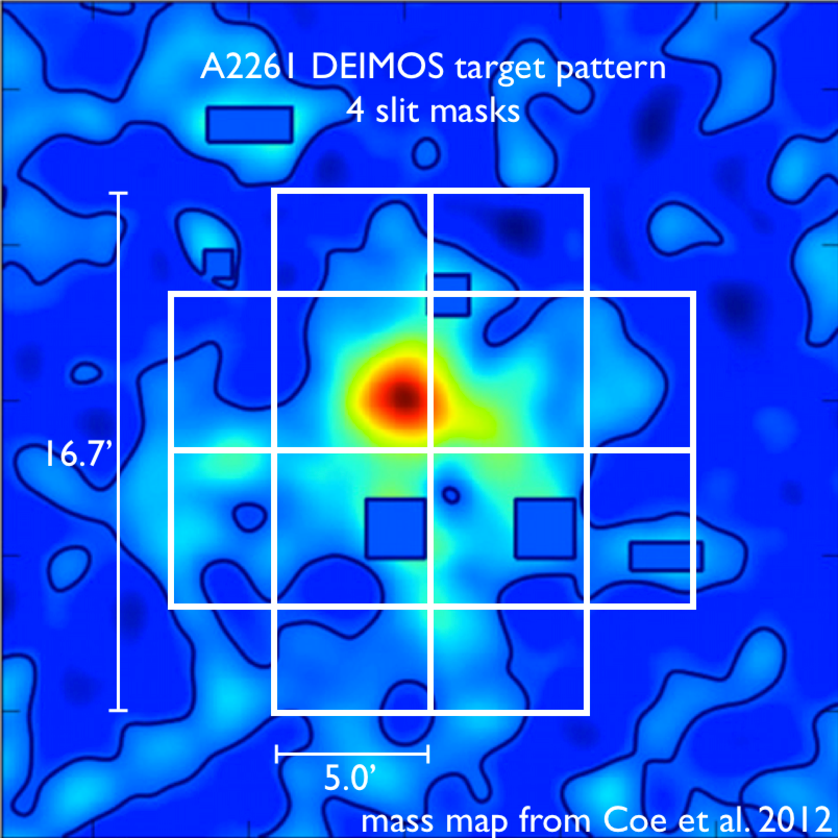
\includegraphics[width=0.85\linewidth]{Plots/a2261_deimos_mask.pdf}
    \caption{\footnotesize Mass map of A2261, with proposed DEIMOS slitmask geometry superposed.}
    \label{fig:maskoverlay}
    \end{center}
  \end{minipage}
\end{figure}


\renewcommand{\bibfont}{\small}
\begin{spacing}{0}
\bibliographystyle{apj}
\bibliography{proposal}
\end{spacing}

\newpage

\section{Technical Remarks}

\subsection{Targets and Exposures}

Abell 2261 (17h22m28.3s +32d09m13s, $z=0.225$, \citealt{Coe2012}) is an ideal target for testing this novel mass mapping technique since its high mass ($M_{\rm vir}\approx 2.2 \times 10^{15}\,M_{\odot}$) and moderate redshift produces a large lensing signal for background galaxies at $z\sim0.6-1.2$, and its angular size $R_{\rm vir} \approx 3\,{\rm Mpc} = 13.4'$ is well-matched to the DEIMOS field of view. We propose to cover this cluster with 4 slit masks, with most of the area covered twice by perpendicular masks to allow repeat observations of targets with $\Delta P.A.=90\degr$ (Figure~\ref{fig:maskoverlay}). This will enable us to measure velocities along both photometric axes to better constrain the shear.

Abell 2261 is part of the CLASH sample \citep{Postman2012} which obtained multi-wavelength HST data for the inner $\sim3'$ and has existing Subaru Suprime-Cam data in B, V, and R bands. We will target galaxies behind the cluster using a color selection modeled on the DEEP2 survey \citep{Newman2013} which successfully identified a large sample of high redshift galaxies and measured rotation curves using the [OII] emission line. To resolve the [OII] doublet from $z\approx0.6-1.2$, we will use the 1200 line/mm grating centered $\lambda=7200$\AA with the GG495 blocking filter. We will use $1"$ slit widths and lengths chosen to extend past the disk turnover radius predicted from the Subaru photometry, aligned with the photometric major or minor axes up to a maximum tilt of $30\degr$.

The line flux needed for measuring kinematics with the DEIMOS configuration used by DEEP2 is $\gtrsim10^{-17}\,{\rm erg/s/cm^2}$ \citep{Kassin2012}. Using COSMOS data \citep{Jouvel2009}, we find that a BVR color selection of resolved ($r_{1/2}>0.5"$) galaxies with exponential surface-brightness profiles from Subaru photometry with a target density of $1.5-2\,{\rm arcmin^{-2}}$ can efficiently select objects at $z\sim0.6-1.2$ with [OII] fluxes above this threshold. This strategy should produce a sample of $>100$ galaxies with two-dimensional kinematics measured at $z_{\rm med}\approx0.8$. To ensure sufficient ${\rm S/N}$ in velocity measurements along both axes, we request \textbf{2 hour exposures $\times$ 4 masks = 8 hours shutter time}, for one night of observations. Because we are targeting a single cluster, it would be preferable to observe over two half-nights to minimize the hour angle. To minimize the effect of differential refraction, we can observe two masks aligned with the parallactic angle during maximum hour angle, and the other two perpendicular masks at minimum.

\subsection{Backup Program}

We will obtain DEIMOS spectroscopy for a fair sample of galaxies to $r$=24.0 in the Sloan Digital Sky Survey South Equatorial Stripe. These redshifts will be used to calibrate photometric redshift estimates in this field which covers $\sim200$ square degrees with extensive multi-wavelength data for extragalactic science and weak lensing.

\subsection{Status of Previously Approved Keck Programs}
The PI (Schlegel) obtained 1 night of LRIS spectroscopy in 2006A and 2 nights on DEIMOS in 2006B. The data from these observations resulted in five refereed publications:

{\small
\begin{description}
  \item {Barbary}, K., {et~al} 2009, ApJ, 690, 1358
  \item {Barbary}, K., {et~al} 2012a, ApJ, 745, 31
  \item {Barbary}, K., {et~al} 2012b, ApJ, 745, 31
  \item {Dawson}, K.~S., {et~al} 2009, AJ,  138, 1271
  \item {Suzuki}, N., {et~al} 2012, ApJ, 746, 85
\end{description}
}

\subsection{Path to Science from Observations}
We will generate wavelength-calibrated, sky-subtracted 2D spectra using the existing DEIMOS spectroscopic reduction software designed for DEEP2; the data expected from this proposal is very similar to that for which this pipeline was originally designed. Rotation curves will be extracted from the 2D spectra in the usual manner, fitting the core spectrum in spatial slices with a psf-convolved line template and marginalizing over the relevant nuisance parameters. For the imaging component of the weak lensing study, we will use a shape measurement pipeline that has already been validated on the HST and Subaru imaging as part of the CLASH project.

\subsection{Technical Concerns}
If our preferred dates for observing Abell 2261 are overscheduled, we can target another CLASH cluster at a different RA, for example MACS1115+0129, Abell 1423 (11h57m), MACS1720+3536, each of which has multi-wavelength Subaru data needed for targeting.

\subsection{Experience and Publications}
The team has extensive experience with optical spectroscopy including development of the spectroscopic pipeline used for SDSS and BOSS which have been applied to numerous extragalactic studies including measurement of the local Tully-Fisher relation. We have also led analyses of DEIMOS spectra as part of the DEEP2 survey, as well as weak lensing studies including shape measurement and the use of observables beyond shear. Finally, the team has substantial experience in the field of lensing by massive galaxy clusters, in particular from the CLASH program. An abbreviated reference list follows, with papers using Lick or Keck data highlighted with an asterisk.

{\small
\begin{description}
\item \textit{Optical spectroscopy and Tully-Fisher analysis:}
  \begin{description}
  \item \** {Mostek}, N., {Coil}, A.~L., {Cooper}, M., {Davis}, M., {Newman}, J.~A., \&
    {Weiner}, B.~J. 2013, ApJ, 767, 89
  \item \** {Mostek}, N., {Coil}, A.~L., {Moustakas}, J., {Salim}, S., \& {Weiner}, B.~J.
    2012, ApJ, 746, 124
  \item {Schlegel}, D., {White}, M., \& {Eisenstein}, D. 2009, in Astronomy, Vol. 2010,
    astro2010: The Astronomy and Astrophysics Decadal Survey, 314
  \item \** {Schlegel}, D.~J. 1995, PhD thesis, UNIVERSITY OF CALIFORNIA, BERKELEY.
  \end{description}
\item \textit{Weak lensing shape measurement and analysis:}
  \begin{description}
  \item {George}, M.~R., {et~al.} 2012, ApJ, 757, 2
  \item {Huff}, E.~M., {Eifler}, T., {Hirata}, C.~M., {Mandelbaum}, R., {Schlegel}, D.,
    \& {Seljak}, U. 2011{\natexlab{a}}, ArXiv e-prints
  \item {Huff}, E.~M., \& {Graves}, G.~J. 2011, ArXiv e-prints
  \item {Huff}, E.~M., {Hirata}, C.~M., {Mandelbaum}, R., {Schlegel}, D., {Seljak}, U.,
    \& {Lupton}, R.~H. 2011{\natexlab{b}}, ArXiv e-prints
  \item {Melchior}, P., {Sutter}, P.~M., {Sheldon}, E.~S., {Krause}, E., \& {Wandelt},
    B.~D. 2013, ArXiv e-prints
  \item {Melchior}, P., {Viola}, M., {Sch{\"a}fer}, B.~M., \& {Bartelmann}, M. 2011,
    MNRAS, 412, 1552
  \end{description}
\item \textit{Weak gravitational lensing by galaxy clusters:}
  \begin{description}
  \item {Coe}, D., {et~al.} 2012, ApJ, 757, 22
  \item Medezinski, E. et al., 2013, ArXiv e-prints (accepted by ApJ)
  \item {Merten}, J., {Cacciato}, M., {Meneghetti}, M., {Mignone}, C., \& {Bartelmann},
    M. 2009, A\&A, 500, 681
  \item Postman, M., et al., 2012, ApJS, 199, 25
  \item Umetsu, K., 2013, ApJ, 769, 13 
  \item Umetsu, K., et al, 2012, ApJ, 755, 56
    \end{description}
\end{description}
}

\subsection{Resources and Publication Timescale}
We have the computational resources and funding needed to carry out this project, and aim to produce rotation velocity measurements within three months, shear estimates within six months, and publications describing the first detection of kinematic weak lensing along with a detailed mass map within one year of observations.

\end{document}